\documentclass[twoside]{book}

% Packages required by doxygen
\usepackage{fixltx2e}
\usepackage{calc}
\usepackage{doxygen}
\usepackage[export]{adjustbox} % also loads graphicx
\usepackage{graphicx}
\usepackage[utf8]{inputenc}
\usepackage{makeidx}
\usepackage{multicol}
\usepackage{multirow}
\PassOptionsToPackage{warn}{textcomp}
\usepackage{textcomp}
\usepackage[nointegrals]{wasysym}
\usepackage[table]{xcolor}

% Font selection
\usepackage[T1]{fontenc}
\usepackage[scaled=.90]{helvet}
\usepackage{courier}
\usepackage{amssymb}
\usepackage{sectsty}
\renewcommand{\familydefault}{\sfdefault}
\allsectionsfont{%
  \fontseries{bc}\selectfont%
  \color{darkgray}%
}
\renewcommand{\DoxyLabelFont}{%
  \fontseries{bc}\selectfont%
  \color{darkgray}%
}
\newcommand{\+}{\discretionary{\mbox{\scriptsize$\hookleftarrow$}}{}{}}

% Page & text layout
\usepackage{geometry}
\geometry{%
  a4paper,%
  top=2.5cm,%
  bottom=2.5cm,%
  left=2.5cm,%
  right=2.5cm%
}
\tolerance=750
\hfuzz=15pt
\hbadness=750
\setlength{\emergencystretch}{15pt}
\setlength{\parindent}{0cm}
\setlength{\parskip}{3ex plus 2ex minus 2ex}
\makeatletter
\renewcommand{\paragraph}{%
  \@startsection{paragraph}{4}{0ex}{-1.0ex}{1.0ex}{%
    \normalfont\normalsize\bfseries\SS@parafont%
  }%
}
\renewcommand{\subparagraph}{%
  \@startsection{subparagraph}{5}{0ex}{-1.0ex}{1.0ex}{%
    \normalfont\normalsize\bfseries\SS@subparafont%
  }%
}
\makeatother

% Headers & footers
\usepackage{fancyhdr}
\pagestyle{fancyplain}
\fancyhead[LE]{\fancyplain{}{\bfseries\thepage}}
\fancyhead[CE]{\fancyplain{}{}}
\fancyhead[RE]{\fancyplain{}{\bfseries\leftmark}}
\fancyhead[LO]{\fancyplain{}{\bfseries\rightmark}}
\fancyhead[CO]{\fancyplain{}{}}
\fancyhead[RO]{\fancyplain{}{\bfseries\thepage}}
\fancyfoot[LE]{\fancyplain{}{}}
\fancyfoot[CE]{\fancyplain{}{}}
\fancyfoot[RE]{\fancyplain{}{\bfseries\scriptsize Generated by Doxygen }}
\fancyfoot[LO]{\fancyplain{}{\bfseries\scriptsize Generated by Doxygen }}
\fancyfoot[CO]{\fancyplain{}{}}
\fancyfoot[RO]{\fancyplain{}{}}
\renewcommand{\footrulewidth}{0.4pt}
\renewcommand{\chaptermark}[1]{%
  \markboth{#1}{}%
}
\renewcommand{\sectionmark}[1]{%
  \markright{\thesection\ #1}%
}

% Indices & bibliography
\usepackage{natbib}
\usepackage[titles]{tocloft}
\setcounter{tocdepth}{3}
\setcounter{secnumdepth}{5}
\makeindex

% Hyperlinks (required, but should be loaded last)
\usepackage{ifpdf}
\ifpdf
  \usepackage[pdftex,pagebackref=true]{hyperref}
\else
  \usepackage[ps2pdf,pagebackref=true]{hyperref}
\fi
\hypersetup{%
  colorlinks=true,%
  linkcolor=blue,%
  citecolor=blue,%
  unicode%
}

% Custom commands
\newcommand{\clearemptydoublepage}{%
  \newpage{\pagestyle{empty}\cleardoublepage}%
}

\usepackage{caption}
\captionsetup{labelsep=space,justification=centering,font={bf},singlelinecheck=off,skip=4pt,position=top}

%===== C O N T E N T S =====

\begin{document}

% Titlepage & ToC
\hypersetup{pageanchor=false,
             bookmarksnumbered=true,
             pdfencoding=unicode
            }
\pagenumbering{roman}
\begin{titlepage}
\vspace*{7cm}
\begin{center}%
{\Large electrotest \\[1ex]\large 0.\+99 }\\
\vspace*{1cm}
{\large Generated by Doxygen 1.8.11}\\
\end{center}
\end{titlepage}
\clearemptydoublepage
\tableofcontents
\clearemptydoublepage
\pagenumbering{arabic}
\hypersetup{pageanchor=true}

%--- Begin generated contents ---
\chapter{File Index}
\section{File List}
Here is a list of all documented files with brief descriptions\+:\begin{DoxyCompactList}
\item\contentsline{section}{libpower/\hyperlink{libpower_8c}{libpower.\+c} \\*Dynamic library for calculating power from resistance or current }{\pageref{libpower_8c}}{}
\item\contentsline{section}{libpower/\hyperlink{libpower_8h}{libpower.\+h} \\*Dynamic library for calculating power from resistance or current }{\pageref{libpower_8h}}{}
\item\contentsline{section}{libpower/\hyperlink{test_8c}{test.\+c} \\*Test program for the libpower library }{\pageref{test_8c}}{}
\end{DoxyCompactList}

\chapter{File Documentation}
\hypertarget{libpower_8c}{}\section{libpower/libpower.c File Reference}
\label{libpower_8c}\index{libpower/libpower.\+c@{libpower/libpower.\+c}}


dynamic library for calculating power from resistance or current.  


{\ttfamily \#include \char`\"{}libpower.\+h\char`\"{}}\\*
Include dependency graph for libpower.\+c\+:\nopagebreak
\begin{figure}[H]
\begin{center}
\leavevmode
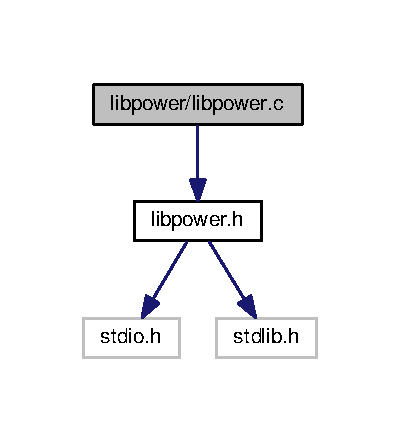
\includegraphics[width=192pt]{libpower_8c__incl}
\end{center}
\end{figure}
\subsection*{Functions}
\begin{DoxyCompactItemize}
\item 
float \hyperlink{libpower_8c_ac075500b29b883b6c3ec6d6d6b91d73c}{calc\+\_\+power\+\_\+r} (float volt, float resistance)
\begin{DoxyCompactList}\small\item\em function to calculate power from voltage and resistance \end{DoxyCompactList}\item 
float \hyperlink{libpower_8c_a1f0fd46c93dd4e37cd60b06026ba174f}{calc\+\_\+power\+\_\+i} (float volt, float current)
\begin{DoxyCompactList}\small\item\em function to calculate power from voltage and current \end{DoxyCompactList}\end{DoxyCompactItemize}


\subsection{Detailed Description}
dynamic library for calculating power from resistance or current. 

\begin{DoxyAuthor}{Author}
Lorenz Gerber 
\end{DoxyAuthor}
\begin{DoxyDate}{Date}
31.\+10.\+2016 
\end{DoxyDate}


\subsection{Function Documentation}
\index{libpower.\+c@{libpower.\+c}!calc\+\_\+power\+\_\+i@{calc\+\_\+power\+\_\+i}}
\index{calc\+\_\+power\+\_\+i@{calc\+\_\+power\+\_\+i}!libpower.\+c@{libpower.\+c}}
\subsubsection[{\texorpdfstring{calc\+\_\+power\+\_\+i(float volt, float current)}{calc_power_i(float volt, float current)}}]{\setlength{\rightskip}{0pt plus 5cm}float calc\+\_\+power\+\_\+i (
\begin{DoxyParamCaption}
\item[{float}]{volt, }
\item[{float}]{current}
\end{DoxyParamCaption}
)}\hypertarget{libpower_8c_a1f0fd46c93dd4e37cd60b06026ba174f}{}\label{libpower_8c_a1f0fd46c93dd4e37cd60b06026ba174f}


function to calculate power from voltage and current 

The function calculates power in watt according to the formula volt$\ast$ current


\begin{DoxyParams}{Parameters}
{\em volt} & float, Voltage in volt \\
\hline
{\em current} & float, current in ampere \\
\hline
\end{DoxyParams}
\begin{DoxyReturn}{Returns}
power float, Power in watt 
\end{DoxyReturn}


Here is the caller graph for this function\+:\nopagebreak
\begin{figure}[H]
\begin{center}
\leavevmode
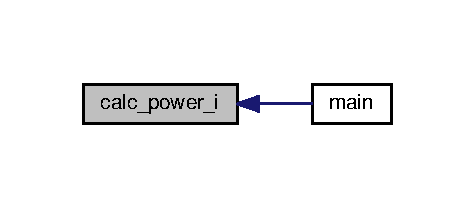
\includegraphics[width=228pt]{libpower_8c_a1f0fd46c93dd4e37cd60b06026ba174f_icgraph}
\end{center}
\end{figure}


\index{libpower.\+c@{libpower.\+c}!calc\+\_\+power\+\_\+r@{calc\+\_\+power\+\_\+r}}
\index{calc\+\_\+power\+\_\+r@{calc\+\_\+power\+\_\+r}!libpower.\+c@{libpower.\+c}}
\subsubsection[{\texorpdfstring{calc\+\_\+power\+\_\+r(float volt, float resistance)}{calc_power_r(float volt, float resistance)}}]{\setlength{\rightskip}{0pt plus 5cm}float calc\+\_\+power\+\_\+r (
\begin{DoxyParamCaption}
\item[{float}]{volt, }
\item[{float}]{resistance}
\end{DoxyParamCaption}
)}\hypertarget{libpower_8c_ac075500b29b883b6c3ec6d6d6b91d73c}{}\label{libpower_8c_ac075500b29b883b6c3ec6d6d6b91d73c}


function to calculate power from voltage and resistance 

The function calculates power in watt according to the formula volt$^\wedge$2/resistance


\begin{DoxyParams}{Parameters}
{\em volt} & float, Voltage in volt \\
\hline
{\em resistance} & float, Resistance in ohm \\
\hline
\end{DoxyParams}
\begin{DoxyReturn}{Returns}
power float, Power in watt 
\end{DoxyReturn}


Here is the caller graph for this function\+:\nopagebreak
\begin{figure}[H]
\begin{center}
\leavevmode
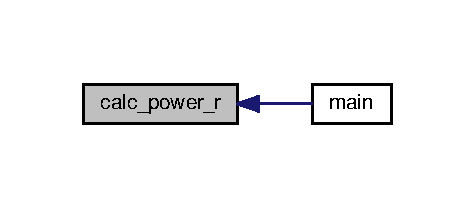
\includegraphics[width=228pt]{libpower_8c_ac075500b29b883b6c3ec6d6d6b91d73c_icgraph}
\end{center}
\end{figure}



\hypertarget{libpower_8h}{}\section{libpower/libpower.h File Reference}
\label{libpower_8h}\index{libpower/libpower.\+h@{libpower/libpower.\+h}}


dynamic library for calculating power from resistance or current.  


{\ttfamily \#include $<$stdio.\+h$>$}\\*
{\ttfamily \#include $<$stdlib.\+h$>$}\\*
Include dependency graph for libpower.\+h\+:\nopagebreak
\begin{figure}[H]
\begin{center}
\leavevmode
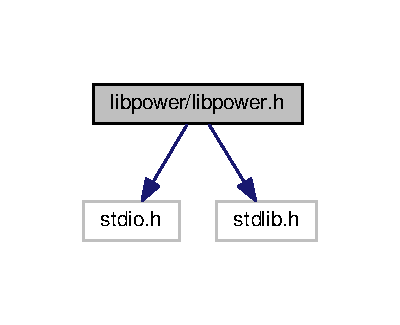
\includegraphics[width=192pt]{libpower_8h__incl}
\end{center}
\end{figure}
This graph shows which files directly or indirectly include this file\+:\nopagebreak
\begin{figure}[H]
\begin{center}
\leavevmode
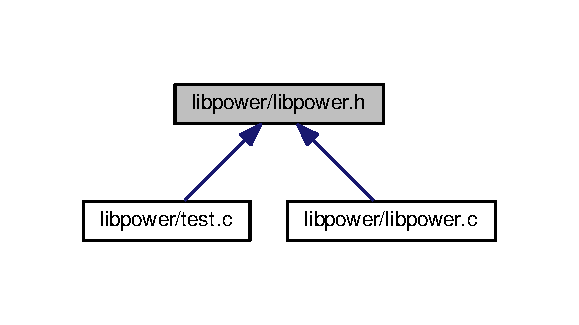
\includegraphics[width=278pt]{libpower_8h__dep__incl}
\end{center}
\end{figure}
\subsection*{Functions}
\begin{DoxyCompactItemize}
\item 
float \hyperlink{libpower_8h_ac075500b29b883b6c3ec6d6d6b91d73c}{calc\+\_\+power\+\_\+r} (float volt, float resistance)
\begin{DoxyCompactList}\small\item\em function to calculate power from voltage and resistance \end{DoxyCompactList}\item 
float \hyperlink{libpower_8h_a1f0fd46c93dd4e37cd60b06026ba174f}{calc\+\_\+power\+\_\+i} (float volt, float current)
\begin{DoxyCompactList}\small\item\em function to calculate power from voltage and current \end{DoxyCompactList}\end{DoxyCompactItemize}


\subsection{Detailed Description}
dynamic library for calculating power from resistance or current. 

\begin{DoxyAuthor}{Author}
Lorenz Gerber 
\end{DoxyAuthor}
\begin{DoxyDate}{Date}
31.\+10.\+2016 
\end{DoxyDate}


\subsection{Function Documentation}
\index{libpower.\+h@{libpower.\+h}!calc\+\_\+power\+\_\+i@{calc\+\_\+power\+\_\+i}}
\index{calc\+\_\+power\+\_\+i@{calc\+\_\+power\+\_\+i}!libpower.\+h@{libpower.\+h}}
\subsubsection[{\texorpdfstring{calc\+\_\+power\+\_\+i(float volt, float current)}{calc_power_i(float volt, float current)}}]{\setlength{\rightskip}{0pt plus 5cm}float calc\+\_\+power\+\_\+i (
\begin{DoxyParamCaption}
\item[{float}]{volt, }
\item[{float}]{current}
\end{DoxyParamCaption}
)}\hypertarget{libpower_8h_a1f0fd46c93dd4e37cd60b06026ba174f}{}\label{libpower_8h_a1f0fd46c93dd4e37cd60b06026ba174f}


function to calculate power from voltage and current 

The function calculates power in watt according to the formula volt$\ast$ current


\begin{DoxyParams}{Parameters}
{\em volt} & float, Voltage in volt \\
\hline
{\em current} & float, current in ampere \\
\hline
\end{DoxyParams}
\begin{DoxyReturn}{Returns}
power float, Power in watt 
\end{DoxyReturn}


Here is the caller graph for this function\+:\nopagebreak
\begin{figure}[H]
\begin{center}
\leavevmode
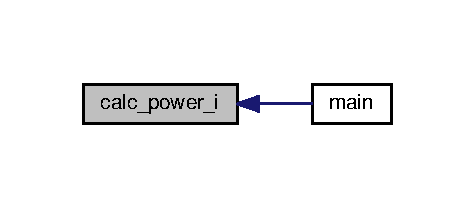
\includegraphics[width=228pt]{libpower_8h_a1f0fd46c93dd4e37cd60b06026ba174f_icgraph}
\end{center}
\end{figure}


\index{libpower.\+h@{libpower.\+h}!calc\+\_\+power\+\_\+r@{calc\+\_\+power\+\_\+r}}
\index{calc\+\_\+power\+\_\+r@{calc\+\_\+power\+\_\+r}!libpower.\+h@{libpower.\+h}}
\subsubsection[{\texorpdfstring{calc\+\_\+power\+\_\+r(float volt, float resistance)}{calc_power_r(float volt, float resistance)}}]{\setlength{\rightskip}{0pt plus 5cm}float calc\+\_\+power\+\_\+r (
\begin{DoxyParamCaption}
\item[{float}]{volt, }
\item[{float}]{resistance}
\end{DoxyParamCaption}
)}\hypertarget{libpower_8h_ac075500b29b883b6c3ec6d6d6b91d73c}{}\label{libpower_8h_ac075500b29b883b6c3ec6d6d6b91d73c}


function to calculate power from voltage and resistance 

The function calculates power in watt according to the formula volt$^\wedge$2/resistance 
\begin{DoxyParams}{Parameters}
{\em volt} & float, Voltage in volt \\
\hline
{\em resistance} & float, Resistance in ohm \\
\hline
\end{DoxyParams}
\begin{DoxyReturn}{Returns}
power float, Power in watt 
\end{DoxyReturn}


Here is the caller graph for this function\+:\nopagebreak
\begin{figure}[H]
\begin{center}
\leavevmode
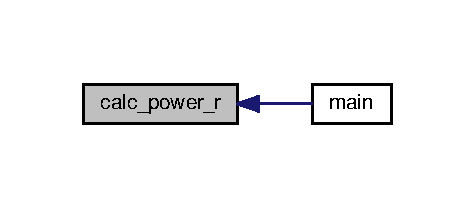
\includegraphics[width=228pt]{libpower_8h_ac075500b29b883b6c3ec6d6d6b91d73c_icgraph}
\end{center}
\end{figure}



\hypertarget{test_8c}{}\section{libpower/test.c File Reference}
\label{test_8c}\index{libpower/test.\+c@{libpower/test.\+c}}


Test program for the libpower library.  


{\ttfamily \#include $<$stdio.\+h$>$}\\*
{\ttfamily \#include \char`\"{}libpower.\+h\char`\"{}}\\*
Include dependency graph for test.\+c\+:\nopagebreak
\begin{figure}[H]
\begin{center}
\leavevmode
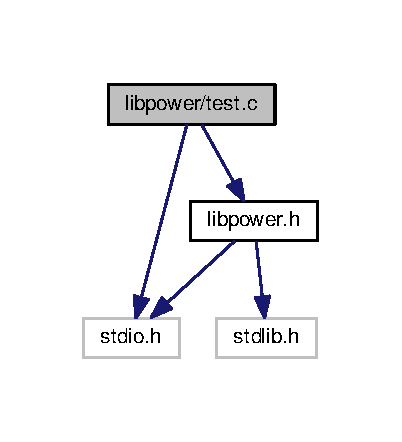
\includegraphics[width=193pt]{test_8c__incl}
\end{center}
\end{figure}
\subsection*{Functions}
\begin{DoxyCompactItemize}
\item 
int \hyperlink{test_8c_a568b3afc214ba30be5bf526d6b27b611}{main} (void)
\end{DoxyCompactItemize}


\subsection{Detailed Description}
Test program for the libpower library. 

\begin{DoxyAuthor}{Author}
Lorenz Gerber 
\end{DoxyAuthor}
\begin{DoxyDate}{Date}
31.\+10.\+2016 
\end{DoxyDate}


\subsection{Function Documentation}
\index{test.\+c@{test.\+c}!main@{main}}
\index{main@{main}!test.\+c@{test.\+c}}
\subsubsection[{\texorpdfstring{main(void)}{main(void)}}]{\setlength{\rightskip}{0pt plus 5cm}main (
\begin{DoxyParamCaption}
\item[{void}]{}
\end{DoxyParamCaption}
)}\hypertarget{test_8c_a568b3afc214ba30be5bf526d6b27b611}{}\label{test_8c_a568b3afc214ba30be5bf526d6b27b611}
this function is used to test the libpower library

This function does not take any command line argument. \begin{DoxyReturn}{Returns}
int, the function returns zero on succes 
\end{DoxyReturn}

%--- End generated contents ---

% Index
\backmatter
\newpage
\phantomsection
\clearemptydoublepage
\addcontentsline{toc}{chapter}{Index}
\printindex

\end{document}
